\part{Hintergrund und Motivation}
\label{part:intro}

\begin{frame}[fragile]{}
\begin{itemize}
	\item HoloLens wie einsetzen?
	\pause
	\item Physik! Physikalische Experimente erweitern
	\pause
	\item Konkretes Experiment als Beispiel nehmen
	\item Anforderungen und Probleme identifizieren und lösen
	\pause
	\item Arbeit schneidet viele Themenbereiche: Computergrafik, MR/AR, Physik, Education, Design, menschliche Wahrnehmung, ... 
\end{itemize}
 
\end{frame}

\part{HoloLens}
\label{part:hololens}
\begin{frame}[fragile]{}
\begin{figure}[h!]
	\centering
	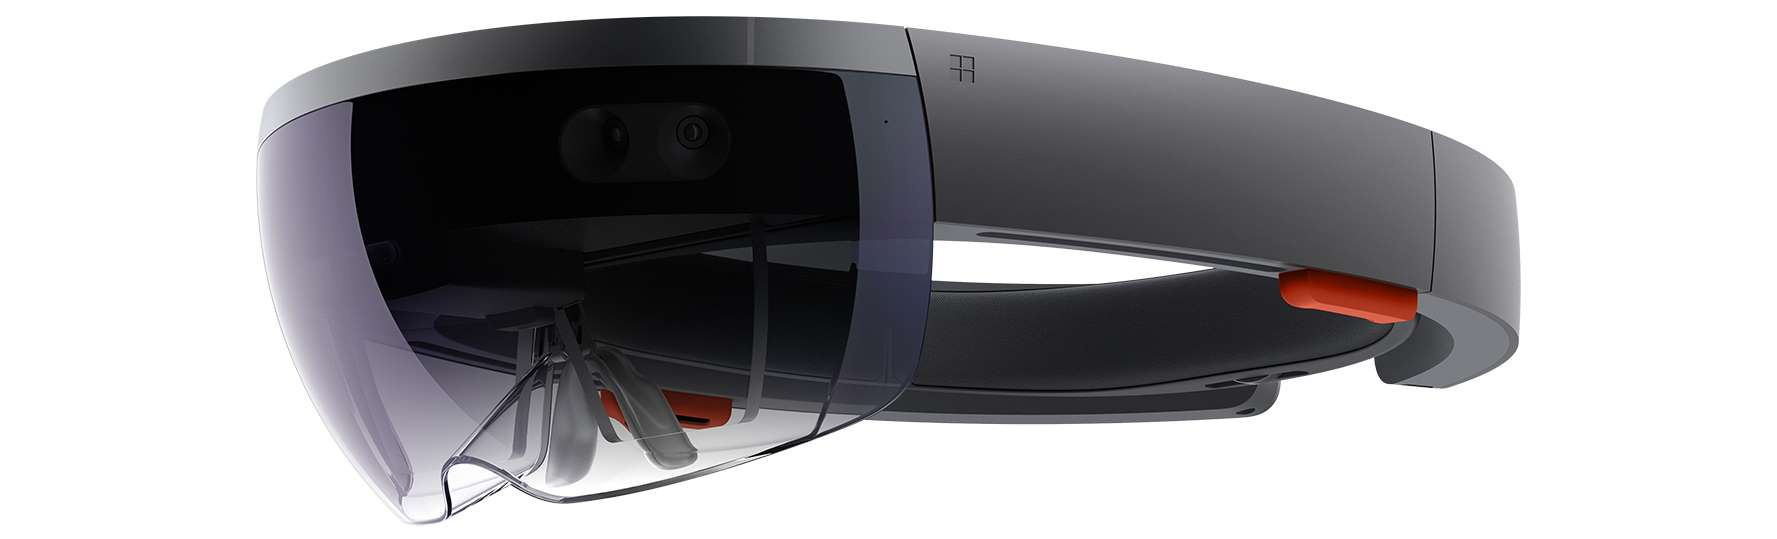
\includegraphics[width=0.7\textwidth]{images/papers/hololens.jpg}
\end{figure}
\begin{itemize}
	\pause
	\item \textit{Augmented Reality} Device
	\pause
	\item Projeziert virtuelle Objekte in das Sichtfeld des Nutzers
	\pause
	\item Nutzer bewegt sich simultan durch reale und virtuelle Szene
	\pause
	\item Genaue Bestimmung von Position und Ausrichtung im Raum durch Sensoren: \textit{Inside-Out-Tracking}
	\pause
	\item Interaktion über Gesten und Sprache
\end{itemize}	
\end{frame}

\begin{frame}[fragile]{}
\begin{figure}[h!]
	\centering
	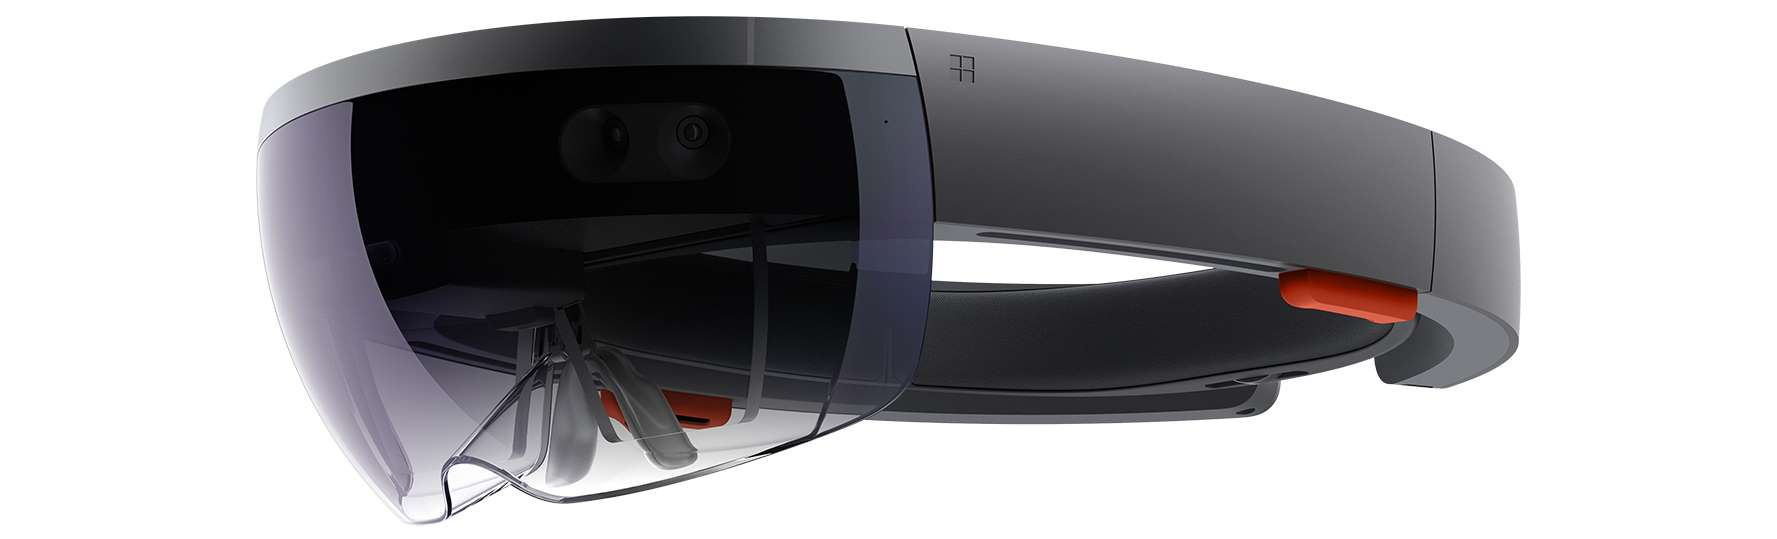
\includegraphics[width=0.5\textwidth]{images/papers/hololens.jpg}
\end{figure}
\begin{itemize}
	\pause
	\item \textit{See-Through, Color Sequential} Display, stereoskopisch, Zwei 16:9 HD Bilder, 32\degree Field of View, 60 Hz Bildwiederholrate hochskaliert auf 240 Hz, Akkomodation der Augen fest bei 2 m
	\pause
	\item \textit{Inside-Out Tracking} über Tiefenkamera (Infrarot), Stereo-Kameras und Inertialmesssystem (IMU)
	\pause
	\item Stand-Alone Device, 1 GHz CPU, 1 GHz HPU, 2 GB RAM, 1 GB HPU RAM, passiv gekühlt, Bluetooth, WiFi
	\pause
	\item Interaktion über Handgesten und englische Sprachkommandos, Cursor = vorwärtsgerichteter Raycast im Zentrum des Sichtfeldes
\end{itemize}	
\end{frame}

\part{State of the Art}
\label{part:sota}
\begin{frame}[fragile]{HoloLens in der Physik}
\begin{figure}
	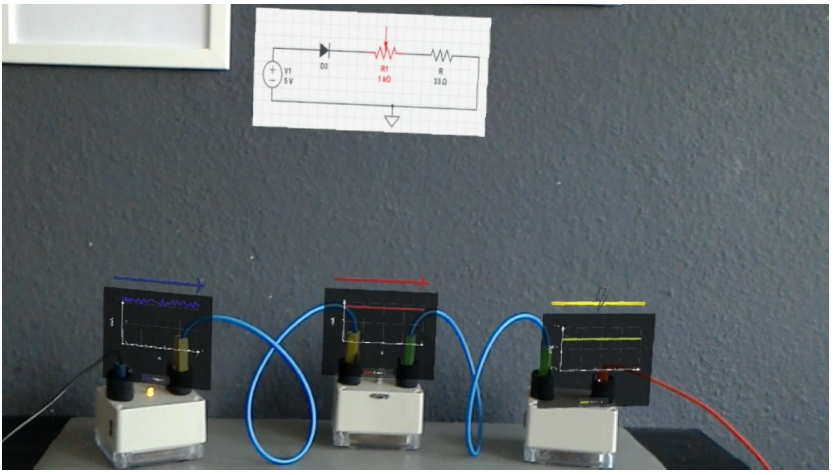
\includegraphics[width=0.43\textwidth]{images/papers/Amiraslanov18.png}
	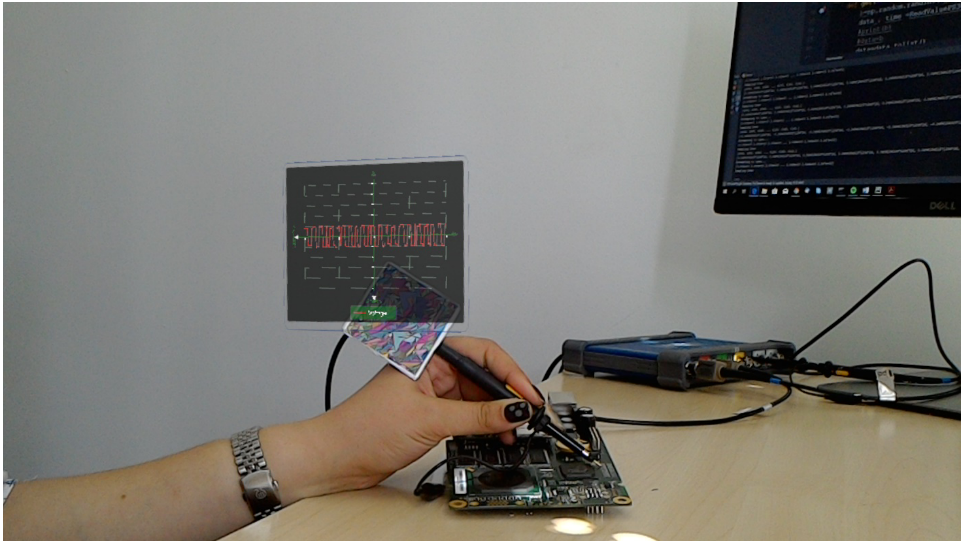
\includegraphics[width=0.43\textwidth]{images/papers/Javaheri18.png}
	\begin{center}
	\vspace{0.05cm}
	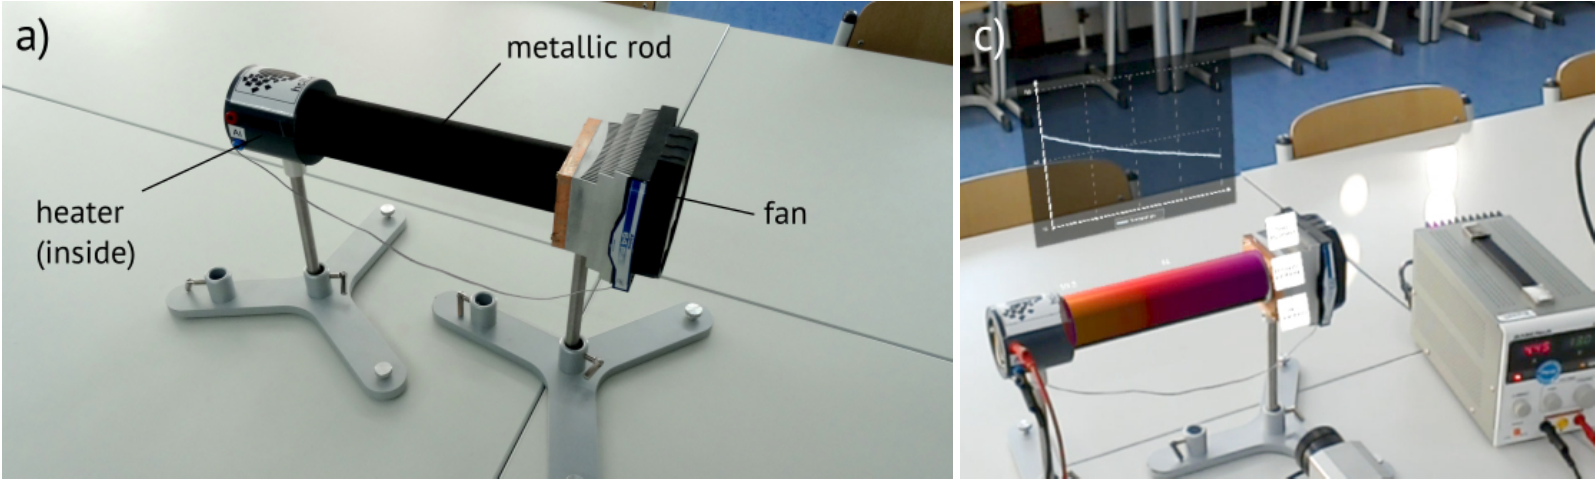
\includegraphics[width=0.87\textwidth]{images/papers/Strzys18.png}	
	\end{center}
	\setlength{\abovecaptionskip}{7pt plus 5pt minus 2pt}
	\caption*{Oben Links: Amiraslanov (2018), Oben Rechts: Javaheri (2018), Unten: Strzys (2017)}
\end{figure}
\end{frame}

\begin{frame}[fragile]{Augmented Reality in der Physik}

\begin{figure}
	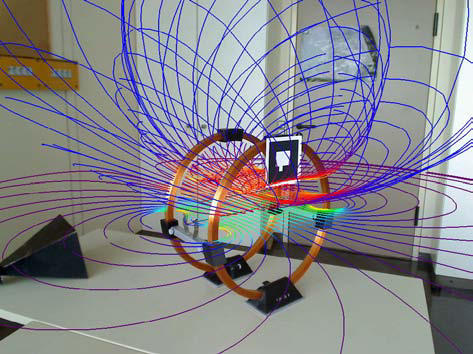
\includegraphics[width=0.35\textwidth]{images/papers/Buchau09.jpg}
	\hspace{0.05cm}
	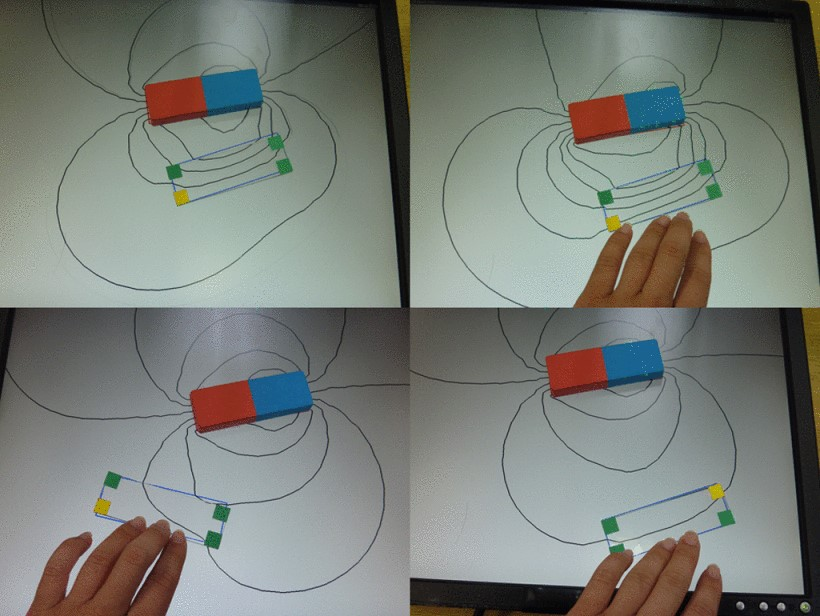
\includegraphics[width=0.35\textwidth]{images/papers/Matsutomo13.jpg}

%	\centering
	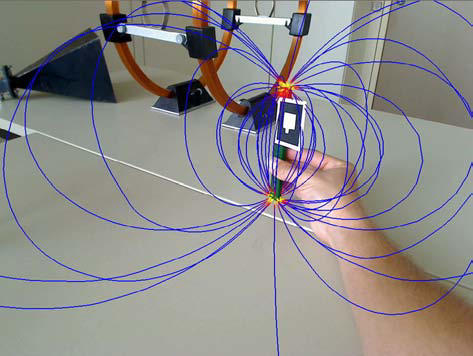
\includegraphics[width=0.35\textwidth]{images/papers/Buchau09_Magnet.jpg}
	\hspace{0.05cm}
	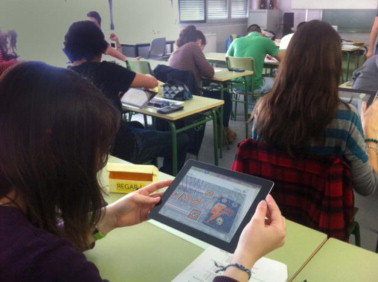
\includegraphics[width=0.35\textwidth]{images/papers/Ibanez14.jpg}

	\setlength{\abovecaptionskip}{5pt plus 5pt minus 2pt}
	\caption*{Links: Buchau (2009), Rechts Oben: Matsutomo (2013), Rechts Unten: Ibanez (2014)}
\end{figure}
\end{frame}

\part{Anwendungsfall: Helmholtz-Spulen}
\label{part:physics}
\begin{frame}[fragile]{Physikalischer Hintergrund}
\begin{minipage}{0.5\textwidth}
	{\setstretch{1.0}
		\begin{itemize}[itemsep=1mm]
			\item Magnetfeld ist 3D-Vektorfeld, Flussdichte $\vec{B}$ in Tesla
			\item Stromfluss durch Spule erzeugt ein Magnetfeld, abhängig von Stromstärke
			\item Helmholtz-Spule: Feld im Inneren weitgehend \textit{homogen}
			\item Feldlinien und Vektormodell sind etablierte Darstellungsmodelle
		\end{itemize}
	}
\end{minipage}
\begin{minipage}{0.45\textwidth}
	\centering
	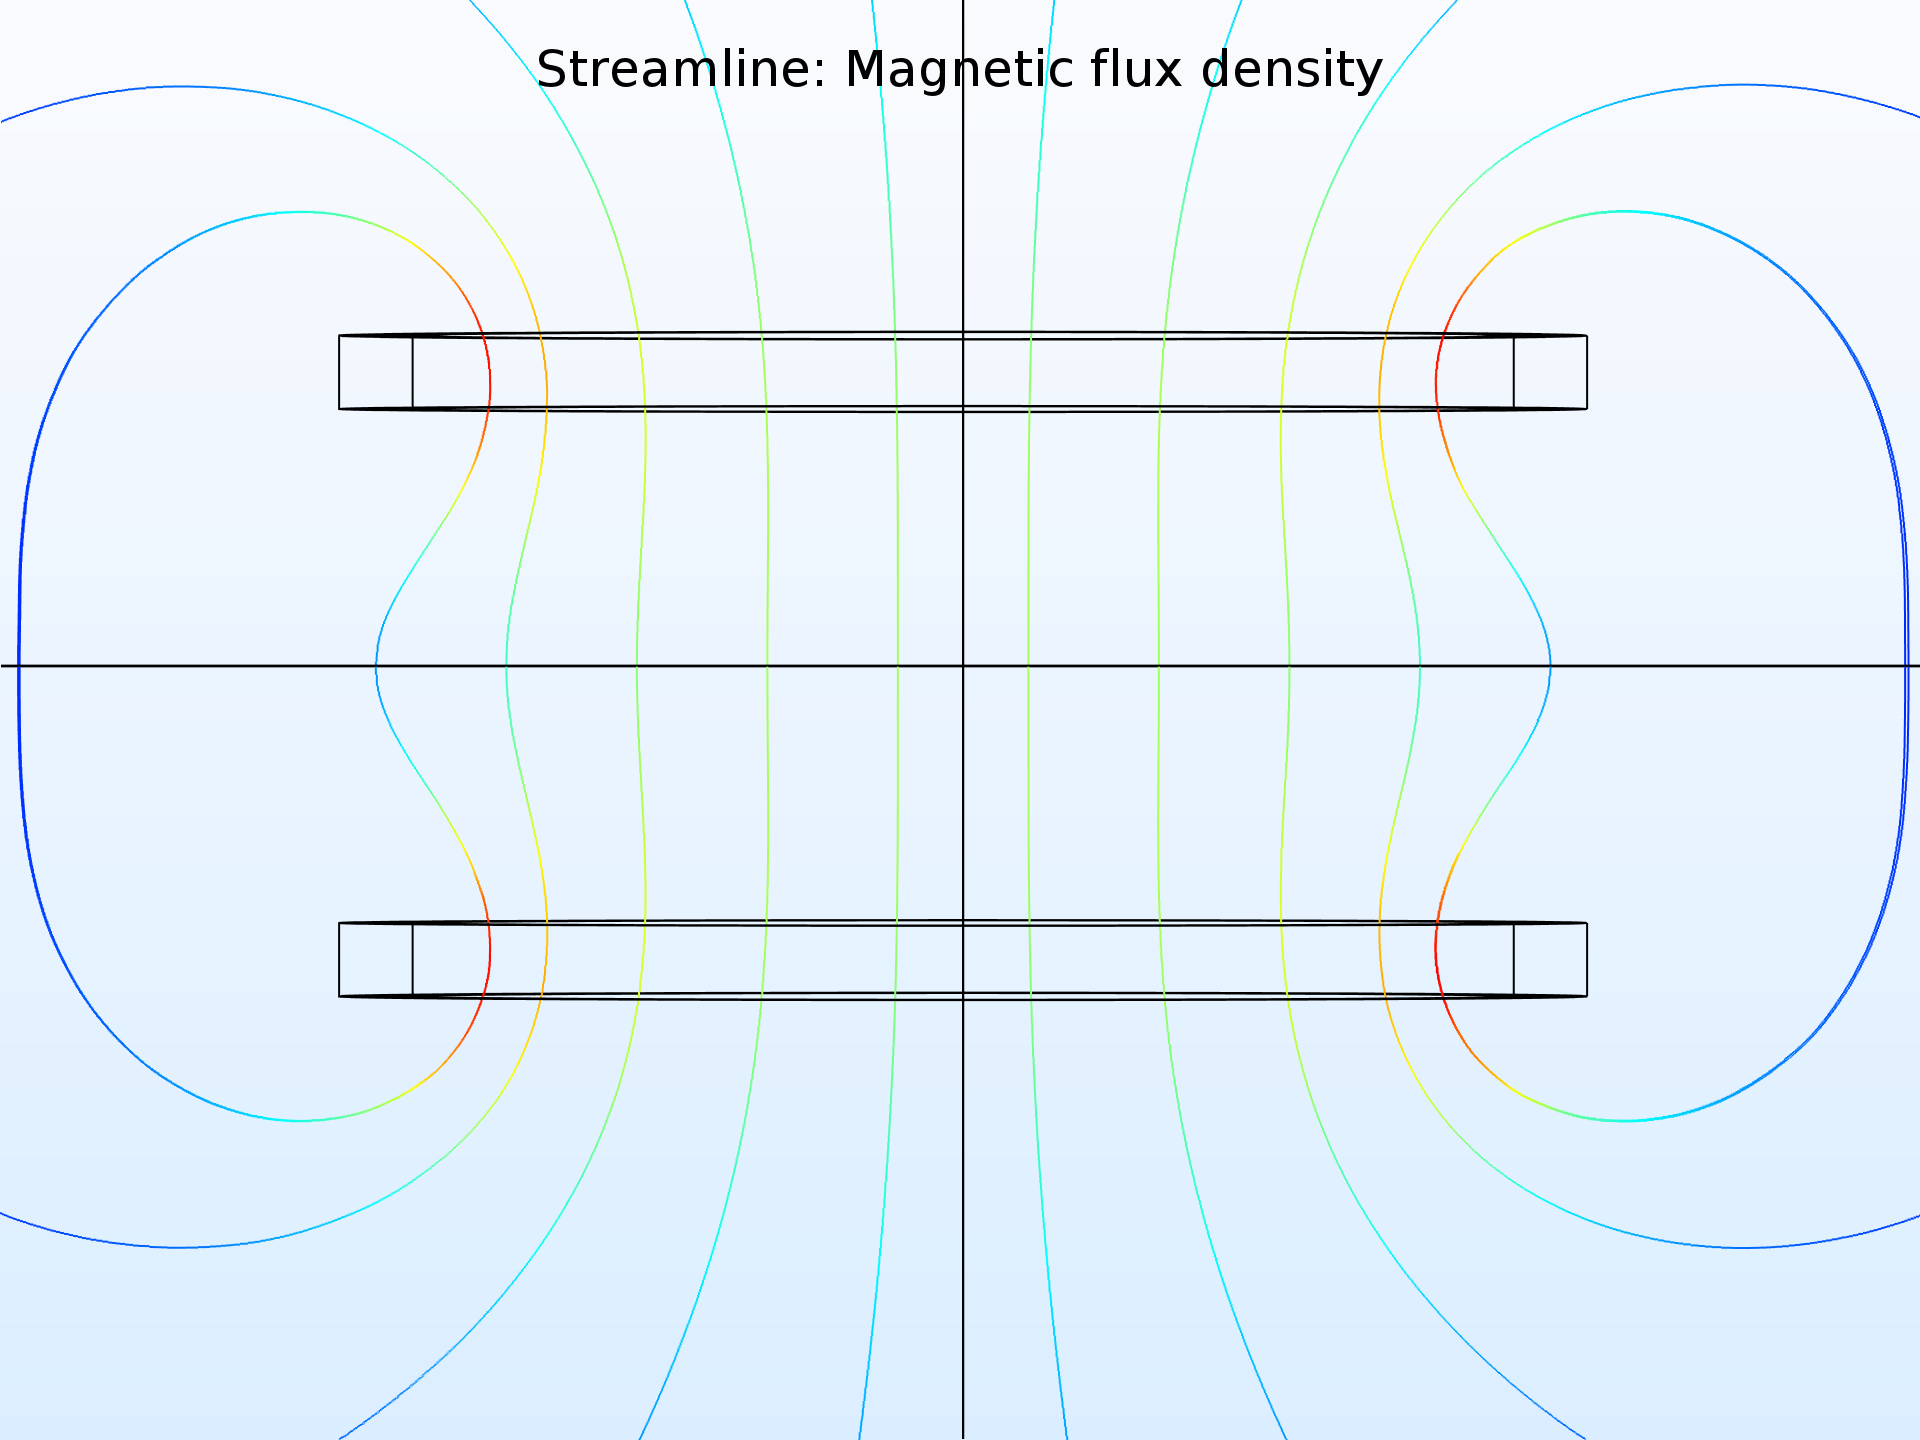
\includegraphics[width=0.9\textwidth]{images/papers/hh_mfield.png}\\
	\small Darstellung des Magnetfeldes einer Helmholtz-Spule mittels Feldlinien für eine Ebene.
\end{minipage}
\end{frame}
\begin{frame}[fragile]{Experiment: Bestimmung des Erdmagnetfeldes}
\begin{minipage}{0.5\textwidth}
	{\setstretch{1.0}
\begin{itemize}[itemsep=1mm]
	\item[$1.$] Kompass ausrichten lassen
	\item[$2.$] Spule orthogonal zur Nord-Süd-Achse aufstellen
	\item[$3.$] Spannungsquelle einschalten und Stromfluss erhöhen, bis Kompassnadel um 45\degree ausgelenkt ist
	\item[$4.$] Flussdichte mit Formel aus Stromstärke und Spuleneigenschaften berechnen
\end{itemize}
}
\end{minipage}
\begin{minipage}{0.45\textwidth}
	\centering
	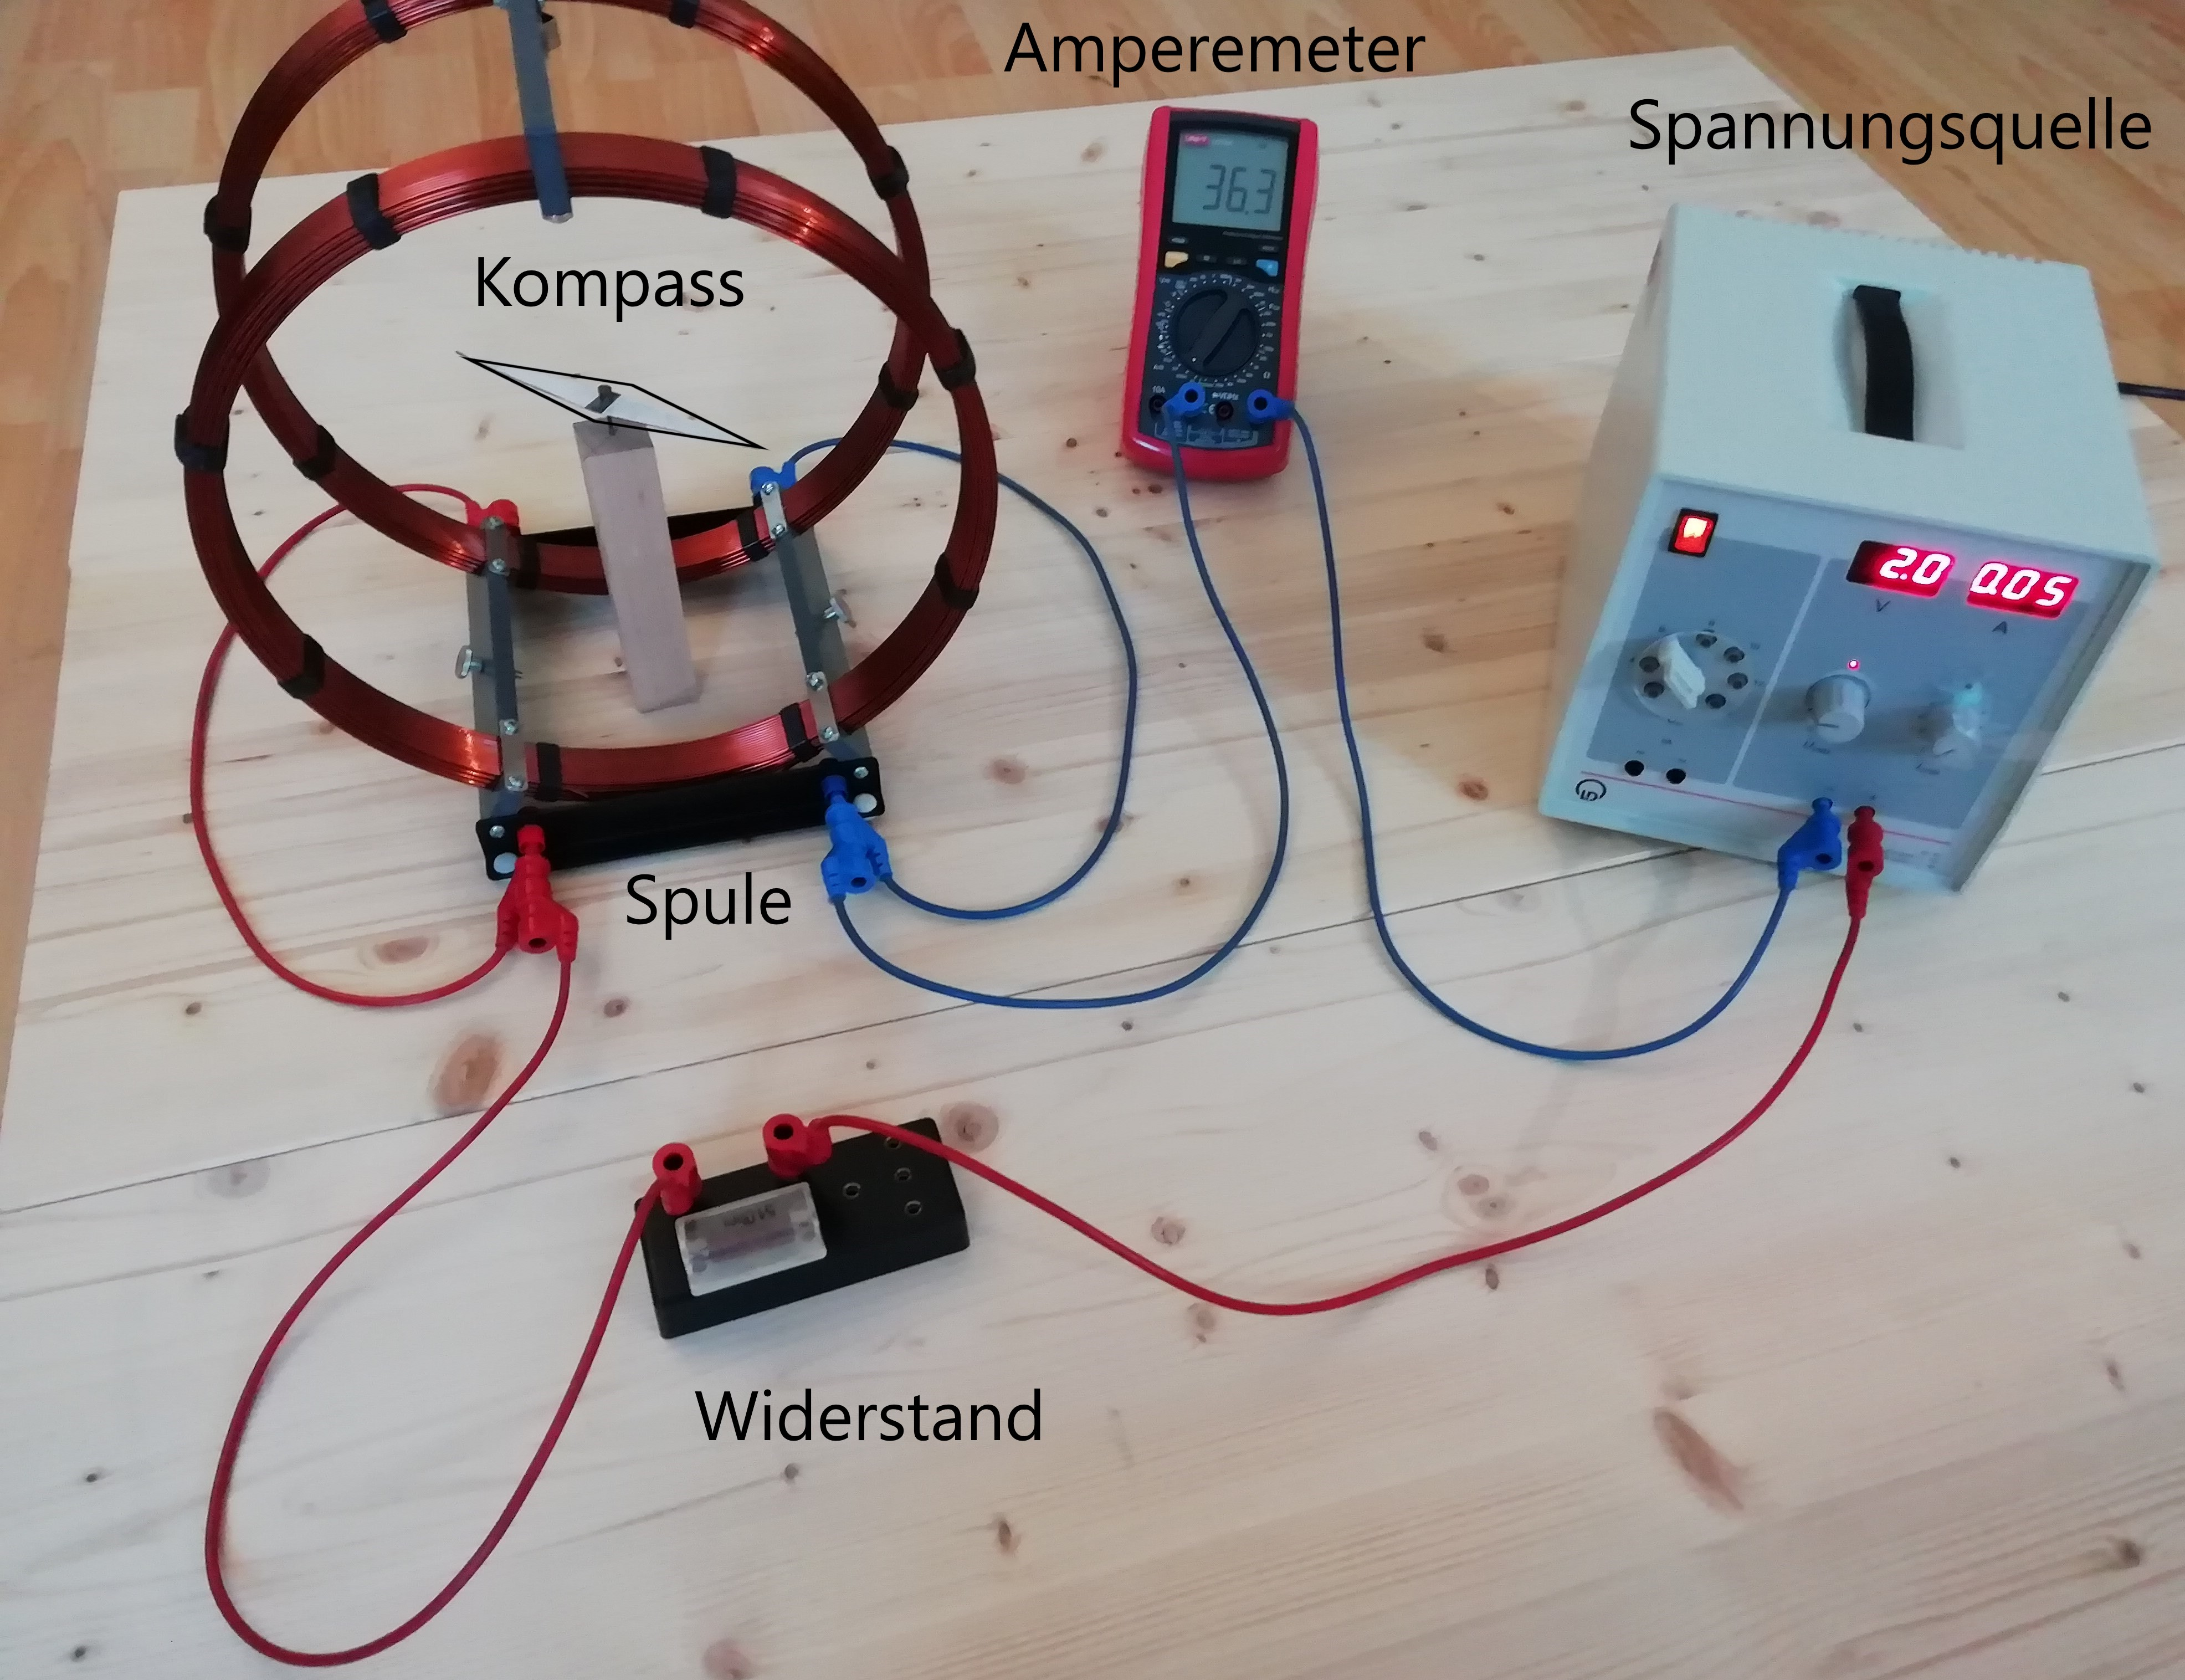
\includegraphics[width=0.9\textwidth]{images/papers/setup_labled.jpg}\\
	\small Foto des Versuchsaufbaus mit Bezeichnung der Elemente.
\end{minipage}
\end{frame}
